%%%%%%%%%%%%%%%%%%%%%%%%%%%%%%%%%%%%%%%%%%%%%%%%%%%%%%%%%%
%%%%%%%%%%%%%%%%%%%%%%%%%%%%%%%%%%%%%%%%%%%%%%%%%%%%%%%%%%
\subsection{Preliminaries}
%%%%%%%%%%%%%%%%%%%%%%%%%%%%%%%%%%%%%%%%%%%%%%%%%%%%%%%%%%
%%%%%%%%%%%%%%%%%%%%%%%%%%%%%%%%%%%%%%%%%%%%%%%%%%%%%%%%%%


%%%%%%%%%%%%%%%%%%%%%%%%%%%%%%%%%%%%%%%%%%%%%%%%%%%%%%%%%%
\frame {\frametitle{Motivations}
%%%%%%%%%%%%%%%%%%%%%%%%%%%%%%%%%%%%%%%%%%%%%%%%%%%%%%%%%%
  \begin{itemize}
  \item \textbf{Examples of graph problems}
    \begin{itemize}
    \item Clustering
    \item Matching problems
    \item Element analysis: node and edge centralities
    \end{itemize}

    \vspace{20pt}
    
  \item \textbf{The problem: big graphs}

    \vspace{20pt}
    
  \item \textbf{Why MapReduce?}
    \begin{itemize}
    \item Algorithms for the above problems on a single machine are
      not scalable
    \item Recently, Google designed a new system, Pregel, for
      large-scale ({\color{red}incremental}) graph processing
    \item Even more recently, \cite{Lattanzi2011} indicate a
      fundamentally new design pattern to analyze graphs in MapReduce
    \item New trend: graph databases, graph processing systems\footnote{If you're interested, we'll discuss this off-line.}
    \end{itemize}
  \end{itemize}
}

%%%%%%%%%%%%%%%%%%%%%%%%%%%%%%%%%%%%%%%%%%%%%%%%%%%%%%%%%%
\frame {\frametitle{Graph Representations}
%%%%%%%%%%%%%%%%%%%%%%%%%%%%%%%%%%%%%%%%%%%%%%%%%%%%%%%%%%
  \begin{itemize}
  \item \textbf{Basic data structures}
    \begin{itemize}
    \item Adjacency matrix
    \item Adjacency list
    \end{itemize}

    \vspace{20pt}

  \item \textbf{Are graphs sparse or dense?}
    \begin{itemize}
    \item Determines which data-structure to use
      \begin{itemize}
      \item Adjacency matrix: operations on incoming links are easy
        (column scan)
      \item Adjacency list: operations on outgoing links are easy
      \item The shuffle and sort phase can help, by grouping edges by
        their destination reducer
      \end{itemize}
    \item \cite{Leskovec2005} dispelled the notion of sparseness of real-world graphs
    \end{itemize}
  \end{itemize}
}

%%%%%%%%%%%%%%%%%%%%%%%%%%%%%%%%%%%%%%%%%%%%%%%%%%%%%%%%%%
%%%%%%%%%%%%%%%%%%%%%%%%%%%%%%%%%%%%%%%%%%%%%%%%%%%%%%%%%%
\subsection{Breadth-First Search}
%%%%%%%%%%%%%%%%%%%%%%%%%%%%%%%%%%%%%%%%%%%%%%%%%%%%%%%%%%
%%%%%%%%%%%%%%%%%%%%%%%%%%%%%%%%%%%%%%%%%%%%%%%%%%%%%%%%%%

%%%%%%%%%%%%%%%%%%%%%%%%%%%%%%%%%%%%%%%%%%%%%%%%%%%%%%%%%%
\frame {\frametitle{Parallel Breadth-First Search}
%%%%%%%%%%%%%%%%%%%%%%%%%%%%%%%%%%%%%%%%%%%%%%%%%%%%%%%%%%
  \begin{itemize}
  \item \textbf{Single-source shortest path}
    \begin{itemize}
    \item Dijkstra algorithm using a {\color{red}global priority
        queue}
      \begin{itemize}
      \item Maintains a globally sorted list of nodes by current distance
      \end{itemize}
   \item How to solve this problem in parallel?
     \begin{itemize}
     \item ``Brute-force'' approach: breadth-first search
     \end{itemize}
    \end{itemize}

    \vspace{40pt}

  \item \textbf{Parallel BFS: intuition}
    \begin{itemize}
    \item Flooding
    \item {\color{red}Iterative algorithm} in MapReduce
    \item Shoehorn message passing style algorithms
    \end{itemize}

  \end{itemize}
}

%%%%%%%%%%%%%%%%%%%%%%%%%%%%%%%%%%%%%%%%%%%%%%%%%%%%%%%%%%
\frame {\frametitle{Parallel Breadth-First Search}
%%%%%%%%%%%%%%%%%%%%%%%%%%%%%%%%%%%%%%%%%%%%%%%%%%%%%%%%%%
  \begin{center}
    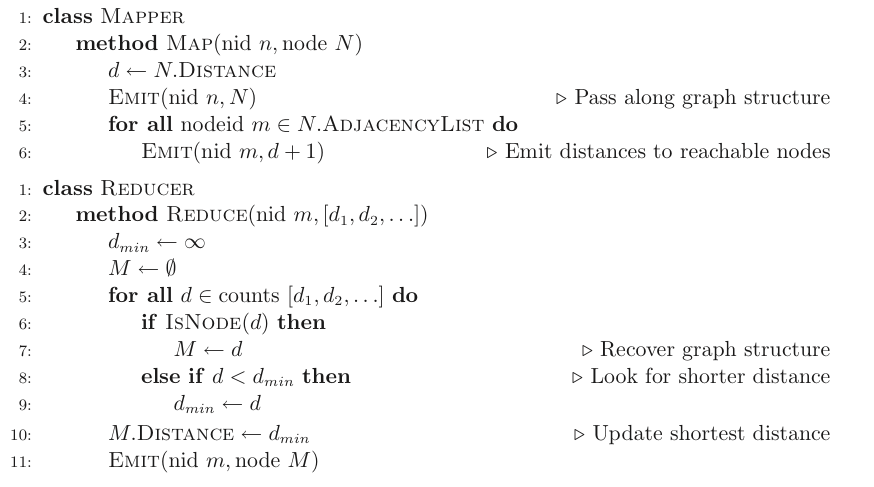
\includegraphics[scale=0.4]{./Figures/pbfs}
  \end{center}
}

%%%%%%%%%%%%%%%%%%%%%%%%%%%%%%%%%%%%%%%%%%%%%%%%%%%%%%%%%%
\frame {\frametitle{Parallel Breadth-First Search}
%%%%%%%%%%%%%%%%%%%%%%%%%%%%%%%%%%%%%%%%%%%%%%%%%%%%%%%%%%
  \begin{itemize}
  \item \textbf{Assumptions}
    \begin{itemize}
    \item Connected, directed graph
    \item Data structure: adjacency list
    \item Distance to each node is stored alongside the adjacency list
      of that node
    \end{itemize}

    \vspace{20pt}

  \item \textbf{The pseudo-code}
    \begin{itemize}
    \item We use $n$ to denote the node id (an integer)
    \item We use $N$ to denote the node adjacency list and current
      distance
    \item The algorithm works by mapping over all nodes
    \item Mappers emit a key-value pair for each neighbor on the
      node's adjacency list
      \begin{itemize}
      \item The key: node id of the neighbor
      \item The value: the current distance to the node plus one
      \item If we can reach node $n$ with a distance $d$, then we must
        be able to reach all the nodes connected to $n$ with distance $d+1$
      \end{itemize}
    \end{itemize}
  \end{itemize}
}

%%%%%%%%%%%%%%%%%%%%%%%%%%%%%%%%%%%%%%%%%%%%%%%%%%%%%%%%%%
\frame {\frametitle{Parallel Breadth-First Search}
%%%%%%%%%%%%%%%%%%%%%%%%%%%%%%%%%%%%%%%%%%%%%%%%%%%%%%%%%%
  \begin{itemize}
  \item \textbf{The pseudo-code (continued)}
    \begin{itemize}
    \item After shuffle and sort, reducers receive keys corresponding
      to the destination node ids and distances corresponding to all
      paths leading to that node
    \item The reducer selects the shortest of these distances and
      update the distance in the node data structure
    \end{itemize}

    \vspace{20pt}

  \item \textbf{Passing the graph along}
    \begin{itemize}
    \item The mapper: emits the node adjacency list, with the node id
      as the key
    \item The reducer: must distinguish between the node data
      structure and the distance values
    \end{itemize}
 \end{itemize}
}

%%%%%%%%%%%%%%%%%%%%%%%%%%%%%%%%%%%%%%%%%%%%%%%%%%%%%%%%%%
\frame {\frametitle{Parallel Breadth-First Search}
%%%%%%%%%%%%%%%%%%%%%%%%%%%%%%%%%%%%%%%%%%%%%%%%%%%%%%%%%%
  \begin{itemize}
  \item \textbf{MapReduce iterations}
    \begin{itemize}
    \item The first time we run the algorithm, we ``discover'' all
      nodes connected to the source
    \item The second iteration, we discover all nodes connected to
      those
    \item[$\to$] Each iteration expands the ``search frontier'' by one
      hop
    \item {\color{red}How many iterations before convergence?}
    \end{itemize}

    \vspace{40pt}

  \item \textbf{This approach is suitable for small-world graphs}
    \begin{itemize}
    \item The diameter of the network is small
    \item See \cite{Lattanzi2011} for advanced topics on the subject
    \end{itemize}
  \end{itemize}
}

%%%%%%%%%%%%%%%%%%%%%%%%%%%%%%%%%%%%%%%%%%%%%%%%%%%%%%%%%%
\frame {\frametitle{Parallel Breadth-First Search}
%%%%%%%%%%%%%%%%%%%%%%%%%%%%%%%%%%%%%%%%%%%%%%%%%%%%%%%%%%
  \begin{itemize}
  \item \textbf{Checking the termination of the algorithm}
    \begin{itemize}
    \item Requires a ``driver'' program which submits a job, check
      termination condition and eventually iterates
    \item In practice:
      \begin{itemize}
      \item Hadoop counters
      \item Side-data to be passed to the job configuration
      \end{itemize}
    \end{itemize}

    \vspace{40pt}

  \item \textbf{Extensions}
    \begin{itemize}
    \item Storing the actual shortest-path
    \item Weighted edges (as opposed to unit distance)
    \end{itemize}
  \end{itemize}
}

%%%%%%%%%%%%%%%%%%%%%%%%%%%%%%%%%%%%%%%%%%%%%%%%%%%%%%%%%%
\frame {\frametitle{The story so far}
%%%%%%%%%%%%%%%%%%%%%%%%%%%%%%%%%%%%%%%%%%%%%%%%%%%%%%%%%%
  \begin{itemize}
  \item \textbf{The graph structure is stored in an adjacency lists}
    \begin{itemize}
    \item This data structure can be augmented with additional information
    \end{itemize}

    \vspace{20pt}

  \item \textbf{The MapReduce framework}
    \begin{itemize}
    \item Maps over the node data structures involving only the node's
      internal state and it's {\color{red}local} graph structure
    \item Map results are ``passed'' along outgoing edges
    \item The graph itself is passed from the mapper to the reducer
      \begin{itemize}
      \item This is a very costly operation for large graphs!
      \end{itemize}
    \item Reducers aggregate over ``same destination'' nodes
    \end{itemize}

    \vspace{20pt}

  \item \textbf{Graph algorithms are generally iterative}
    \begin{itemize}
    \item Require a driver program to check for termination
    \end{itemize}
  \end{itemize}
}

%%%%%%%%%%%%%%%%%%%%%%%%%%%%%%%%%%%%%%%%%%%%%%%%%%%%%%%%%%
%%%%%%%%%%%%%%%%%%%%%%%%%%%%%%%%%%%%%%%%%%%%%%%%%%%%%%%%%%
\subsection{PageRank}
%%%%%%%%%%%%%%%%%%%%%%%%%%%%%%%%%%%%%%%%%%%%%%%%%%%%%%%%%%
%%%%%%%%%%%%%%%%%%%%%%%%%%%%%%%%%%%%%%%%%%%%%%%%%%%%%%%%%%

%%%%%%%%%%%%%%%%%%%%%%%%%%%%%%%%%%%%%%%%%%%%%%%%%%%%%%%%%%
\frame {\frametitle{Introduction}
%%%%%%%%%%%%%%%%%%%%%%%%%%%%%%%%%%%%%%%%%%%%%%%%%%%%%%%%%%
  \begin{itemize}
  \item \textbf{What is PageRank}
    \begin{itemize}
    \item It's a measure of the relevance of a Web page, based on the
      structure of the hyperlink graph
    \item Based on the concept of random Web surfer
    \end{itemize}

    \vspace{20pt}
  
  \item \textbf{Formally we have: }
    $$P(n) = \alpha \Big( \frac{1}{|G|}\Big) + (1-\alpha) \sum_{m \in L(n)}\frac{P(m)}{C(m)}$$
    \begin{itemize}
    \item $|G|$ is the number of nodes in the graph
    \item $\alpha$ is a random jump factor
    \item $L(n)$ is the set of out-going links from page $n$
    \item $C(m)$ is the out-degree of node $m$
    \end{itemize}
  \end{itemize}
}

%%%%%%%%%%%%%%%%%%%%%%%%%%%%%%%%%%%%%%%%%%%%%%%%%%%%%%%%%%
\frame {\frametitle{PageRank in Details}
%%%%%%%%%%%%%%%%%%%%%%%%%%%%%%%%%%%%%%%%%%%%%%%%%%%%%%%%%%
  \begin{itemize}
  \item \textbf{PageRank is defined recursively, hence we need an
      iterative algorithm}
    \begin{itemize}
    \item A node receives ``contributions'' from all pages that link
      to it
    \end{itemize}

    \vspace{20pt}
    
  \item \textbf{Consider the set of nodes $L(n)$}
    \begin{itemize}
    \item A random surfer at $m$ arrives at $n$ with probability
      $1/C(m)$
    \item Since the PageRank value of $m$ is the probability that the
      random surfer is at $m$, the probability of arriving at $n$ from
      $m$ is $P(m)/C(m)$
    \end{itemize}

    \vspace{20pt}

  \item \textbf{To compute the PageRank of $n$ we need:}
    \begin{itemize}
    \item Sum the contributions from all pages that link to $n$
    \item Take into account the random jump, which is uniform over all
      nodes in the graph
    \end{itemize}
  \end{itemize}
}

%%%%%%%%%%%%%%%%%%%%%%%%%%%%%%%%%%%%%%%%%%%%%%%%%%%%%%%%%%
\frame {\frametitle{PageRank in MapReduce}
%%%%%%%%%%%%%%%%%%%%%%%%%%%%%%%%%%%%%%%%%%%%%%%%%%%%%%%%%%
  \begin{center}
    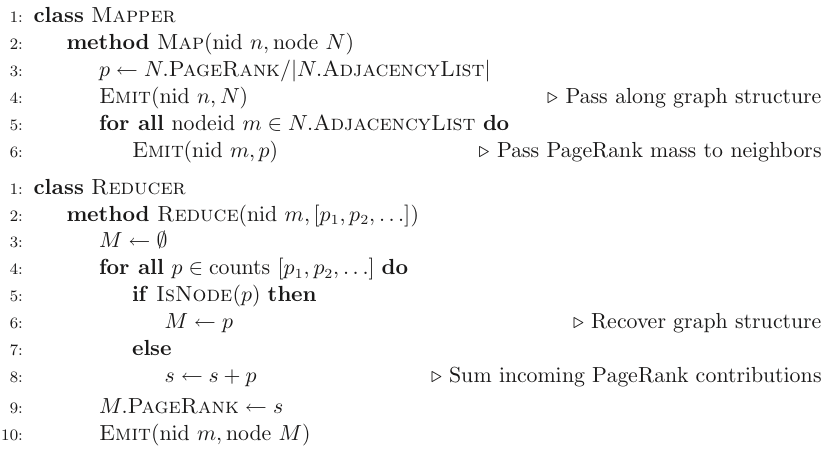
\includegraphics[scale=0.4]{./Figures/pr}
  \end{center}
}

%%%%%%%%%%%%%%%%%%%%%%%%%%%%%%%%%%%%%%%%%%%%%%%%%%%%%%%%%%
\frame {\frametitle{PageRank in MapReduce}
%%%%%%%%%%%%%%%%%%%%%%%%%%%%%%%%%%%%%%%%%%%%%%%%%%%%%%%%%%
  \begin{center}
    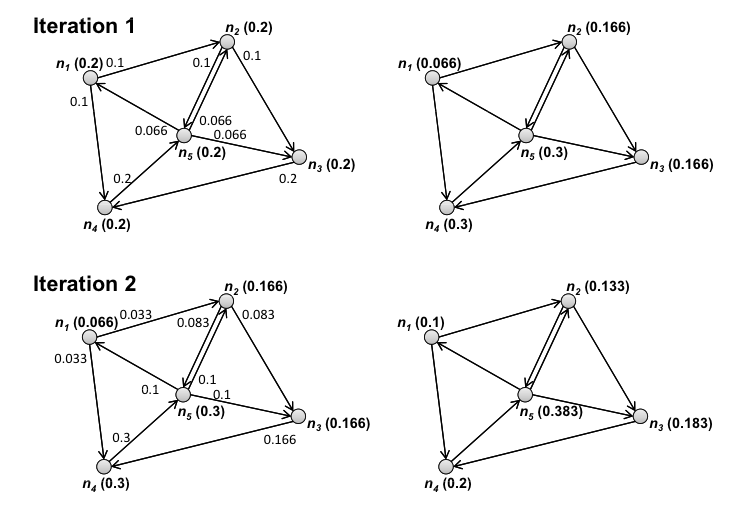
\includegraphics[scale=0.4]{./Figures/pr_toy}
  \end{center}
}

%%%%%%%%%%%%%%%%%%%%%%%%%%%%%%%%%%%%%%%%%%%%%%%%%%%%%%%%%%
\frame {\frametitle{PageRank in MapReduce}
%%%%%%%%%%%%%%%%%%%%%%%%%%%%%%%%%%%%%%%%%%%%%%%%%%%%%%%%%%
 \begin{center}
    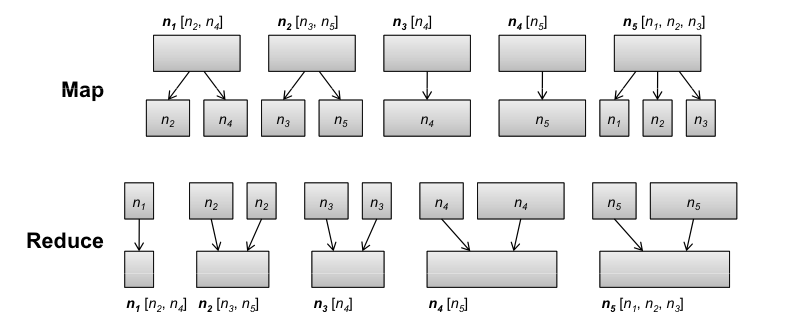
\includegraphics[scale=0.4]{./Figures/pr_sketch}
  \end{center}
}

%%%%%%%%%%%%%%%%%%%%%%%%%%%%%%%%%%%%%%%%%%%%%%%%%%%%%%%%%%
\frame {\frametitle{PageRank in MapReduce}
%%%%%%%%%%%%%%%%%%%%%%%%%%%%%%%%%%%%%%%%%%%%%%%%%%%%%%%%%%
  \begin{itemize}
  \item \textbf{Sketch of the MapReduce algorithm}
    \begin{itemize}
    \item The algorithm maps over the nodes
    \item For each node computes the PageRank mass the needs to be
      distributed to neighbors
    \item Each fraction of the PageRank mass is emitted as the value,
      keyed by the node ids of the neighbors
    \item In the shuffle and sort, values are grouped by node id
      \begin{itemize}
      \item Also, we pass the graph structure from mappers to reducers
        (for subsequent iterations to take place over the updated graph)
      \end{itemize}
    \item The reducer updates the value of the PageRank of every
      single node
    \end{itemize}
  \end{itemize}
}

%%%%%%%%%%%%%%%%%%%%%%%%%%%%%%%%%%%%%%%%%%%%%%%%%%%%%%%%%%
\frame {\frametitle{PageRank in MapReduce}
%%%%%%%%%%%%%%%%%%%%%%%%%%%%%%%%%%%%%%%%%%%%%%%%%%%%%%%%%%
  \begin{itemize}
  \item \textbf{Implementation details}
    \begin{itemize}
    \item Loss of PageRank mass for sink nodes
    \item Auxiliary state information
    \item One iteration of the algorithm
      \begin{itemize}
      \item Two MapReduce jobs: one to distribute the PageRank mass,
        the other for dangling nodes and random jumps
      \end{itemize}
    \item Checking for convergence
      \begin{itemize}
      \item Requires a driver program
      \item When updates of PageRank are ``stable'' the algorithm stops
      \end{itemize}
    \end{itemize}
    
    \vspace{20pt}
    
  \item \textbf{Further reading on {\color{red}convergence} and
      {\color{red}attacks}}
    \begin{itemize}
    \item Convergence: \cite{Page1999, Bianchini2005}
    \end{itemize}
  \end{itemize}
}
